% !TeX root = ../main.tex

\section{Introduzione}
Nei precedenti capitoli sono stati introdotti i concetti alla base della cultura DevOps, del ciclo di vita del processo di sviluppo di applicazioni mobile e delle applicazioni multipiattaforma, arrivando a definire un caso di studio industriale. In questo capitolo viene descritto come è stato effettivamente realizzato il sistema per l'automazione del processo di sviluppo nel rispetto dei requisiti e delle specifiche indicate nel capitolo precedente.

In questa fase di realizzazione del sistema di automazione e di implementazione della pipeline viene considerato il progetto base\footnote{\href{https://github.com/paganellif/DevOps-per-applicazioni-mobile-un-caso-di-studio-industriale/tree/3-applicazioni-multipiattaforma/kmm-example}{https://github.com/paganellif/DevOps-per-applicazioni-mobile-un-caso-di-studio-industriale/tree/3-applicazioni-multipiattaforma/kmm-example}} fornito dal plugin KMM\footnote{\href{https://plugins.jetbrains.com/plugin/14936-kotlin-multiplatform-mobile}{https://plugins.jetbrains.com/plugin/14936-kotlin-multiplatform-mobile}} per Android Studio al fine di mantenere il focus sul processo in modo più agnostico possibile rispetto ad una specifica applicazione utilizzatrice come può essere MaggioliEbook, argomento trattato nel capitolo successivo.


\section{Modello di branching}
L’utilizzo di un adeguato flusso di lavoro è fondamentale per definire una efficiente automazione CI/CD. Con branching si intende l’utilizzo di uno o più flussi principali dai quali divergono altri flussi per svolgere determinati lavori per poi convergere al loro termine: in base alle modalità di apertura e chiusura di questi flussi si definiscono diversi modelli di branching.

Il modello che si intende utilizzare (fig. \ref{branching}) è basato sul modello di branching GitFlow\footnote{\href{https://www.atlassian.com/it/git/tutorials/comparing-workflows/gitflow-workflow}{https://www.atlassian.com/it/git/tutorials/comparing-workflows/gitflow-workflow}} e prevede tre branch principali:

\begin{itemize}
    \item \textbf{dev} - Flusso principale di sviluppo. Ogni modifica apportata a questo branch corrisponde al rilascio di una nuova versione \textit{alpha} per la validazione interna. E' da questo branch che vengono aperti e chiusi nuovi branch, sia per lo sviluppo di nuove funzionalità (\textit{feature}) che per la risoluzione di bug/patch (\textit{fix}).
    \item \textbf{test} - Branch modificato solamente tramite merge di modifiche provenienti dal branch \textit{dev} con lo scopo di rilasciare una nuova versione \textit{beta} per la validazione esterna.
    \item \textbf{main} - Branch modificato solamente tramite merge di modifiche provenienti dal branch \textit{test} con lo scopo di rilasciare una nuova versione in produzione (\textit{prod}).
\end{itemize}

\begin{figure}[H]
    \centering
    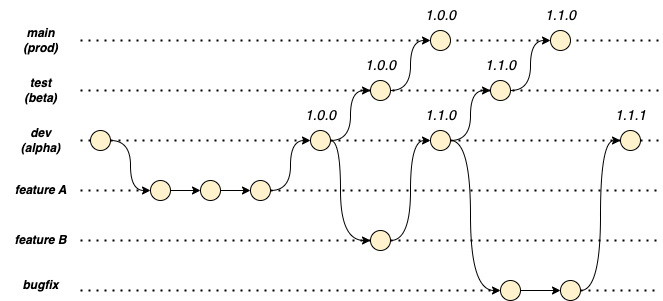
\includegraphics[width=0.7\textwidth]{img/branching-model.png}
    \caption{Esempio di flusso di sviluppo adottando il modello di branching indicato}
    \label{branching}
\end{figure}

Grazie ai meccanismi di automazione a supporto della CI/CD fornite dal CI Server si definiscono specifiche regole di attivazione, chiamate \textit{trigger rules}, che permettono di indicare quando uno specifico job deve essere eseguito. Queste regole si basano su eventi che si verificano sul sistema di versionamento come ad esempio commit, tag e merge request. Tramite questa funzionalità è possibile dunque discriminare quali file sono stati modificati e su quale branch per eseguire le operazioni associate come descritto sopra.

\begin{figure}[H]
    \centering
    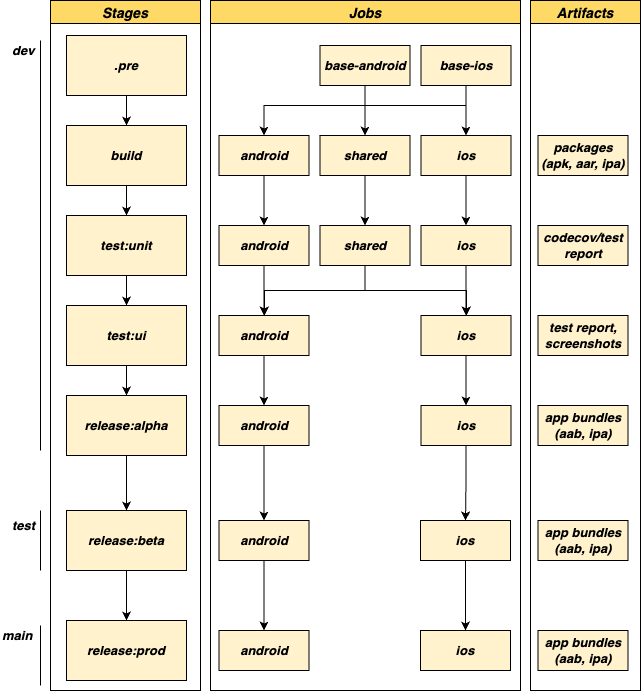
\includegraphics[width=0.8\textwidth]{img/cicd-branch-jobs.png}
    \caption{Stage, job e artefatti associati agli eventi sui branch che compongono l'intera pipeline}
\end{figure}

\section{Continuous Integration}
% progettazione e implementazione CI

\subsection{Build e Packaging}

\subsection{Testing}

\subsection{Dependency Management}

\section{Continuous Delivery}
% progettazione e implementazione CD

\subsection{Alpha/Beta Release}

\section{Continuous Inspection}
% progettazione e implementazione analisi

\section{Templating}
% strumenti utilizzati per favorire il riuso della cicd realizzata

\section{Self-Hosted MacOS GitLab Runner}
% runner macos: in azienda non esistono runner macos.. riprendere il problema del fatto che apple obbliga a usare macOS, indicare le possibili soluzioni (runner managed/self-hosted, ecc) e come ho configurato il runner self-hosted
% approfondire tipologie di runner executor in gitlab e perche ho usato l'executor shell